\clearpage
\chapter{Mini Project 4}

\section{Machine Learning}
\horizontalline{0}{0}

In this Mini-Project, we will build and share machine learning models using Google's `Teachable Machine'.

\subsection*{Learning Goals:}

\begin{itemize}
    \item Explore and build a meaningful Machine Learning Tool from a user perspective.
    \item Identify and demonstrate aspects of a meaningful machine learning project.
    \item Share and test your model with others in the class.
    \item Document your own process of learning to use the tool.
    \item Review and try out models from the class.
\end{itemize}

\subsection*{The Project:}

\noindent Begin by visiting the project website \href{https://teachablemachine.withgoogle.com/}{Teachable Machine 1.0}. \vspace*{1em}

\noindent And watch the intro video \href{https://www.youtube.com/watch?v=T2qQGqZxkD0&t=3s}{Teachable Machine 2.0}. \vspace*{1em}

For this project you will make and share your own meaningful/non-trivial Why meaningful? It should not be a trivial model. It should have a purpose or clear goal - something more than “Does this person 
have a hand on their head?”

\subsection*{Example}

Watch the Pottery demo videos in Moodle. And a current example of how this is currently being used in archaeology. \href{https://www.sciencedaily.com/releases/2021/05/210517144704.htm}{Science Daily}. \vspace*{1em}

\noindent Submit in Gradescope.

% Problem 1
\begin{problem}{Problem 1}
    \begin{statement}{Problem Statement}
        Use the Teachable machine website and picture from the web (or your own) to make a simple “Is this a dog or a human?” model just using images from the web. On this page (fill page) Describe 
        your process of learning how to use the site/tool. How did you choose images? Tricky? Fun? Worked? Include the link to your model.
    \end{statement}

    \begin{Highlight}[Solution]
        \begin{spacing}{1.50}
            The link to my teachable model can be found at \href{https://teachablemachine.withgoogle.com/models/seDY1zadK/}{Dog / Human Model}.
            
            For this part of the project, I first went to Google and downloaded 10 pictures of dogs. I then made sure to review all of the images and make sure that they were clear and obvious pictures 
            of dogs (nothing in the background that could confuse the training of the model). I wanted to make sure that the model had clear and obvious pictures of dogs so that if I fed it a test image
            it would be more likely to correctly identify the images that I fed to the model after being trained.

            I then moved on to doing the same thing for people where I Googled pictures of people (mostly celebrities). Just like when I trained the model with the dogs, I decided to feed it images
            that were clear and distinct images of people with nothing else in the image. I did this for 10 pictures as well and then moved on to testing the model with other pictures that were fed to the
            model.

            After teaching the model, I went to Google and searched for images that weren't initially used to train the model. The first test that I fed to the model was of a picture of a dog in a pasture.
            After feeding the model with this first test image it correctly identified the image as a dog with a 99 \% confidence rate. I found this to be pretty interesting because to a humans eye it was
            clearly a dog and nothing else.

            After doing the first test of the model I did the same test with a human where there was nothing else in the background. Interestingly enough, the model correctly identified that the image
            was of a human. In fact it came back with a 100 \% confidence rate. Of course, to a humans eye this was pretty obvious so it was really cool to see that the model was so confident it what it was
            identifying.

            For the last test, I fed the model a picture of a human and a dog together. After feeding this image to the model the model actually said that the image was a dog with 93 \% confidence. Which
            was interesting, because if I were to guess what the model would return would be a confidence rate of 50 \% because both of models training data was present in the image. But that was clearly not
            the case.

            After going through this activity, it is clear and obvious that the model is pretty reliable for identifying images that are just images of the training data alone. When coupling the two together,
            the model is not as reliable. I think this could be overcame by feeding the model more training data so that it would be even more reliable. I think this is obviously true because this is the core
            tenant of how machine learning works. Models that have less data are going to be less reliable than models that have more.
        \end{spacing}
        \vspace*{-0.5em}
    \end{Highlight}
\end{problem}

% Problem 2
\begin{problem}{Problem 2}
    \begin{statement}{Problem Statement}
        Decide on your own model to create and how you improved it. What makes your model non-trivial? Why did you choose it? It can be any of the three types from the site - Image, Audio, or Movement. 
        Two page narrative here and on pages 3/4. You may include thumbnails of images.
    \end{statement}

    \begin{Highlight}[Solution]
        \begin{spacing}{1.50}
            The link to my teachable model can be found at \href{https://teachablemachine.withgoogle.com/models/dkkzS5pWK/}{Hand Gestures Model}.

            For my own model, I wanted to create a model that would test images, particularly hand gestures. I decided that I wanted to do this because I noticed how accurate the previous model was
            with just still images. In this model, I trained it with three different hand gestures.

            The first hand gesture that I trained the model with was with the oh so popular rock and roll hand gesture. The second hand gesture that I trained the model with was with the peace sign.
            And the last hand gesture that I trained the model with was with the Spock hand from Star Trek. 

            When training this model, I made sure to take a sufficient amount of images that would be used to train the model. For each one of these gestures I made sure to train for each gesture for
            a total of 30 seconds. Each one of these models was about 750 images. Also, a really important aspect of this model was that it was trained with just my right hand and I never changed to
            my left hand.

            For references sake, the model was trained with hand gestures that looked something like this.
            
            \begin{center}
                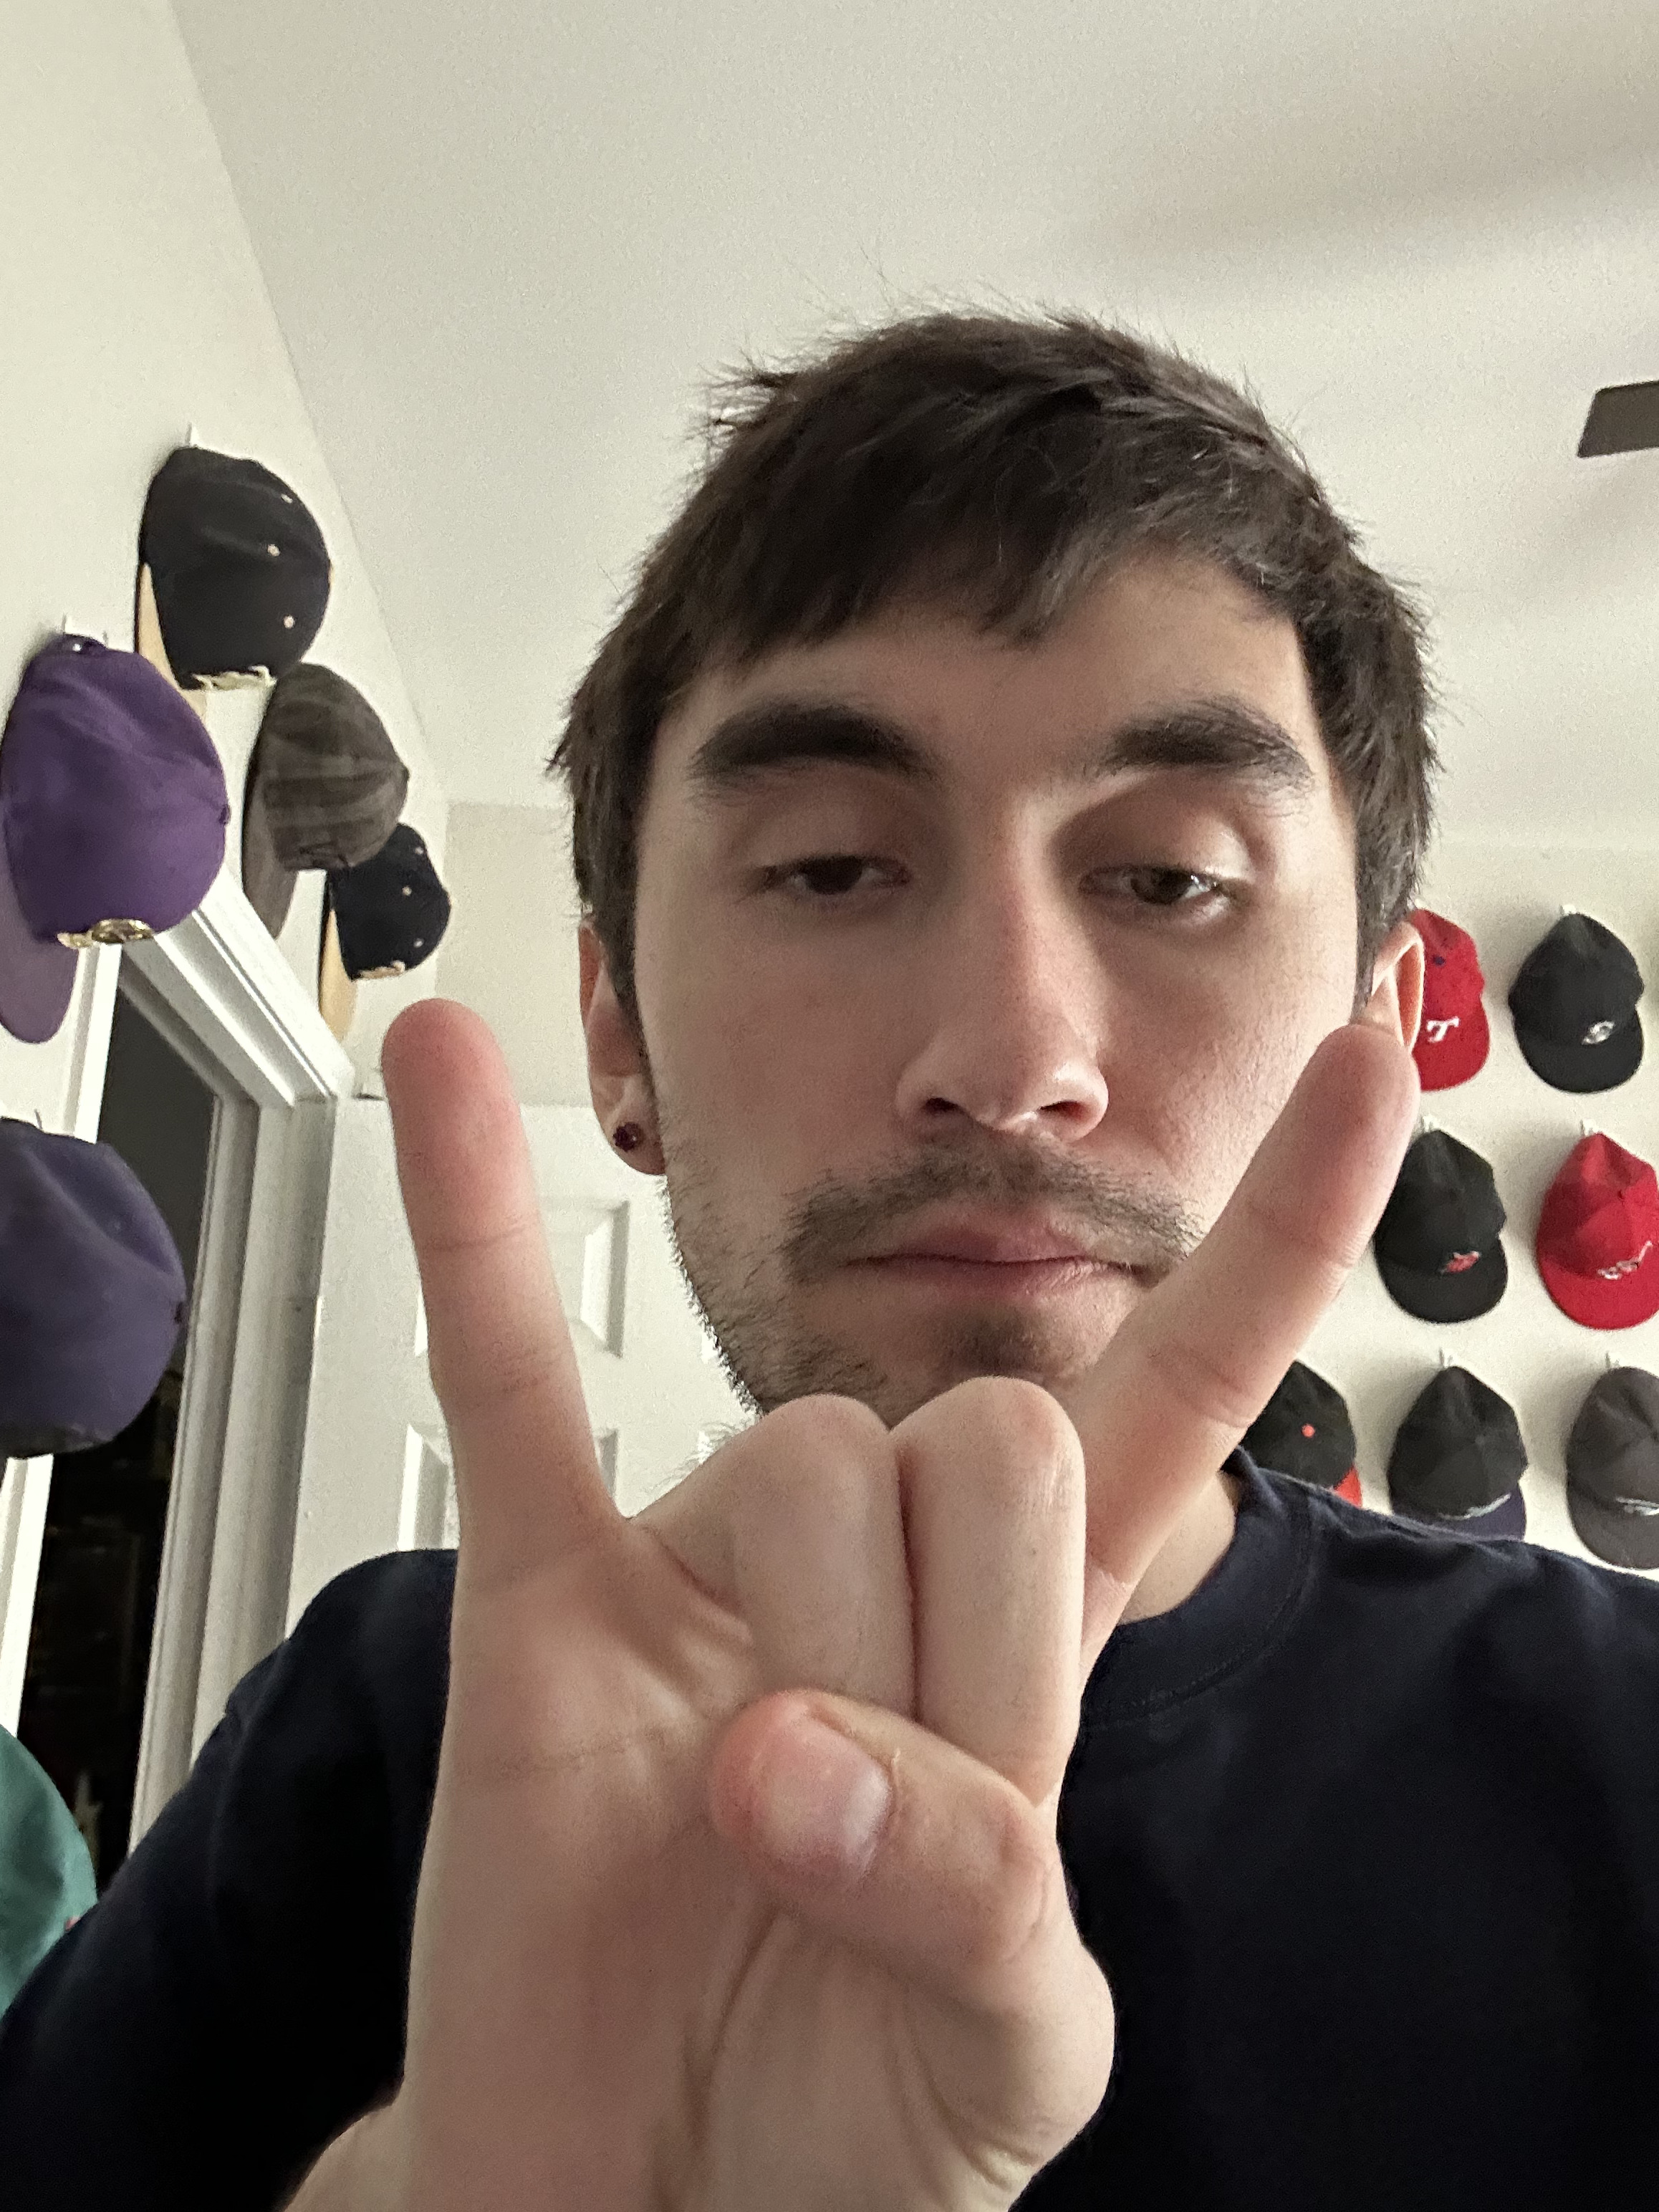
\includegraphics[width = 0.30\textwidth]{./Images/Model 2/Training Images/Rock And Roll.jpg}
                \hspace*{10pt}
                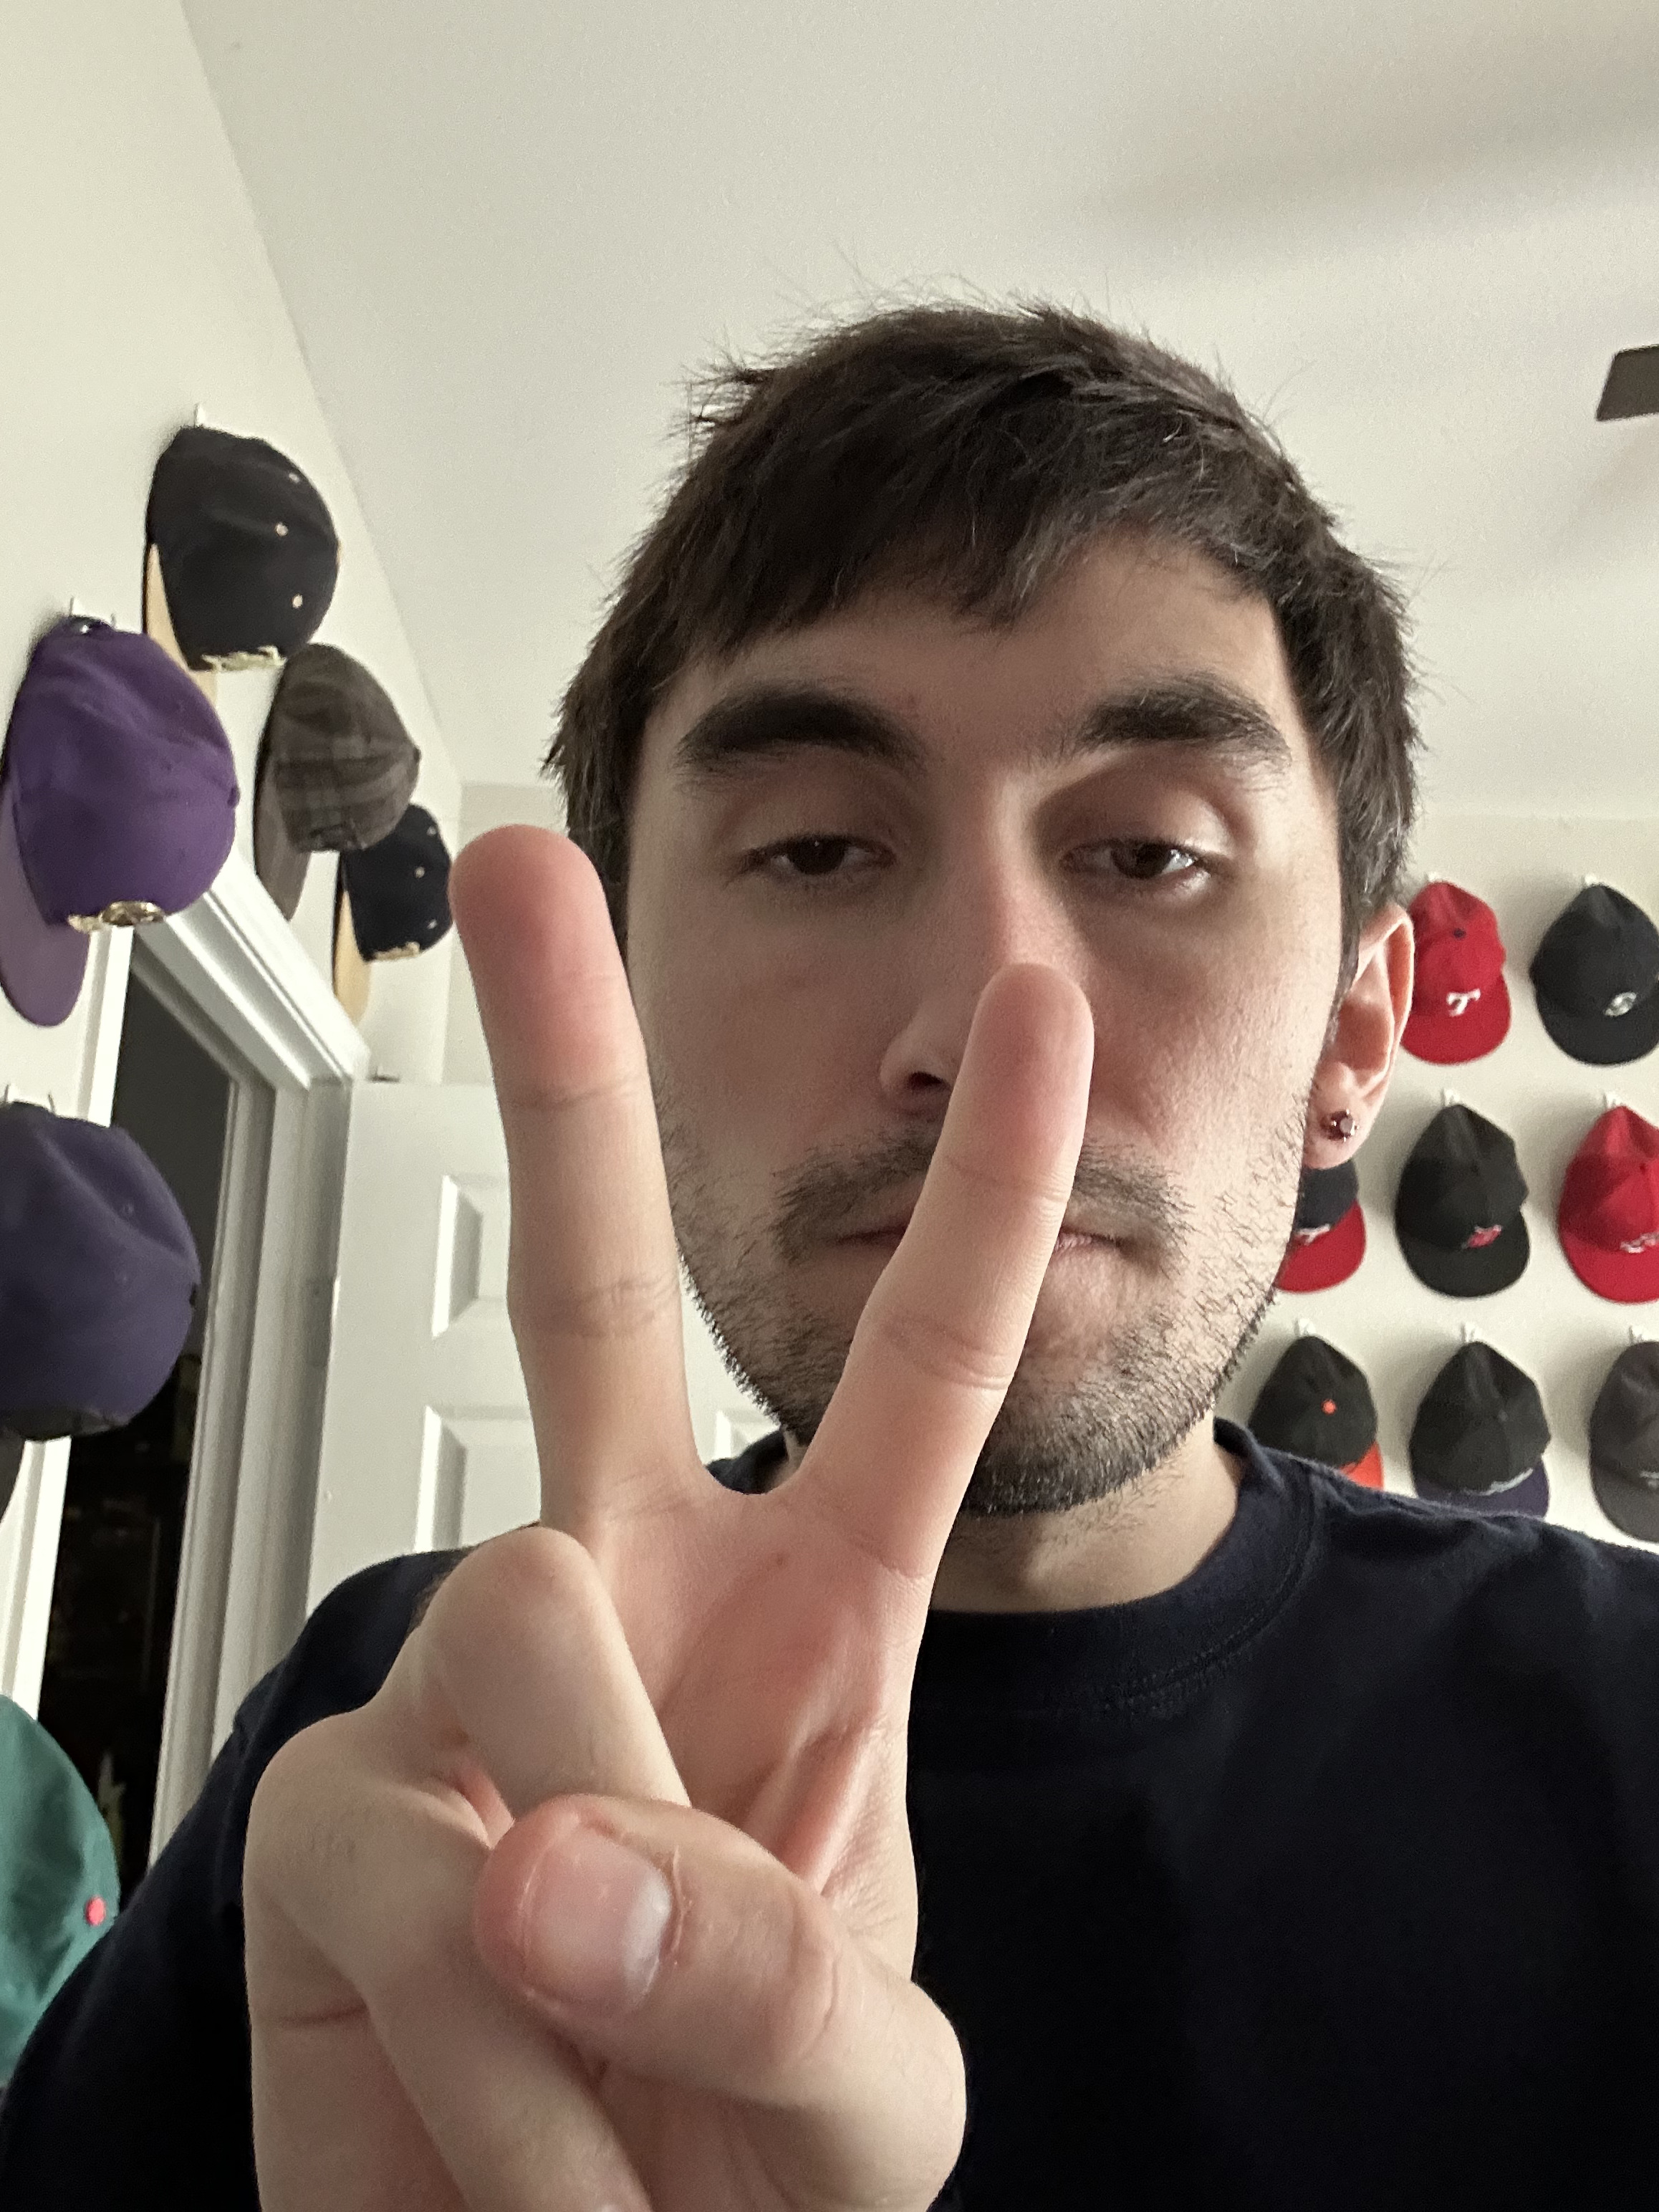
\includegraphics[width = 0.30\textwidth]{./Images/Model 2/Training Images/Peace Sign.jpg}
                \hspace*{10pt}
                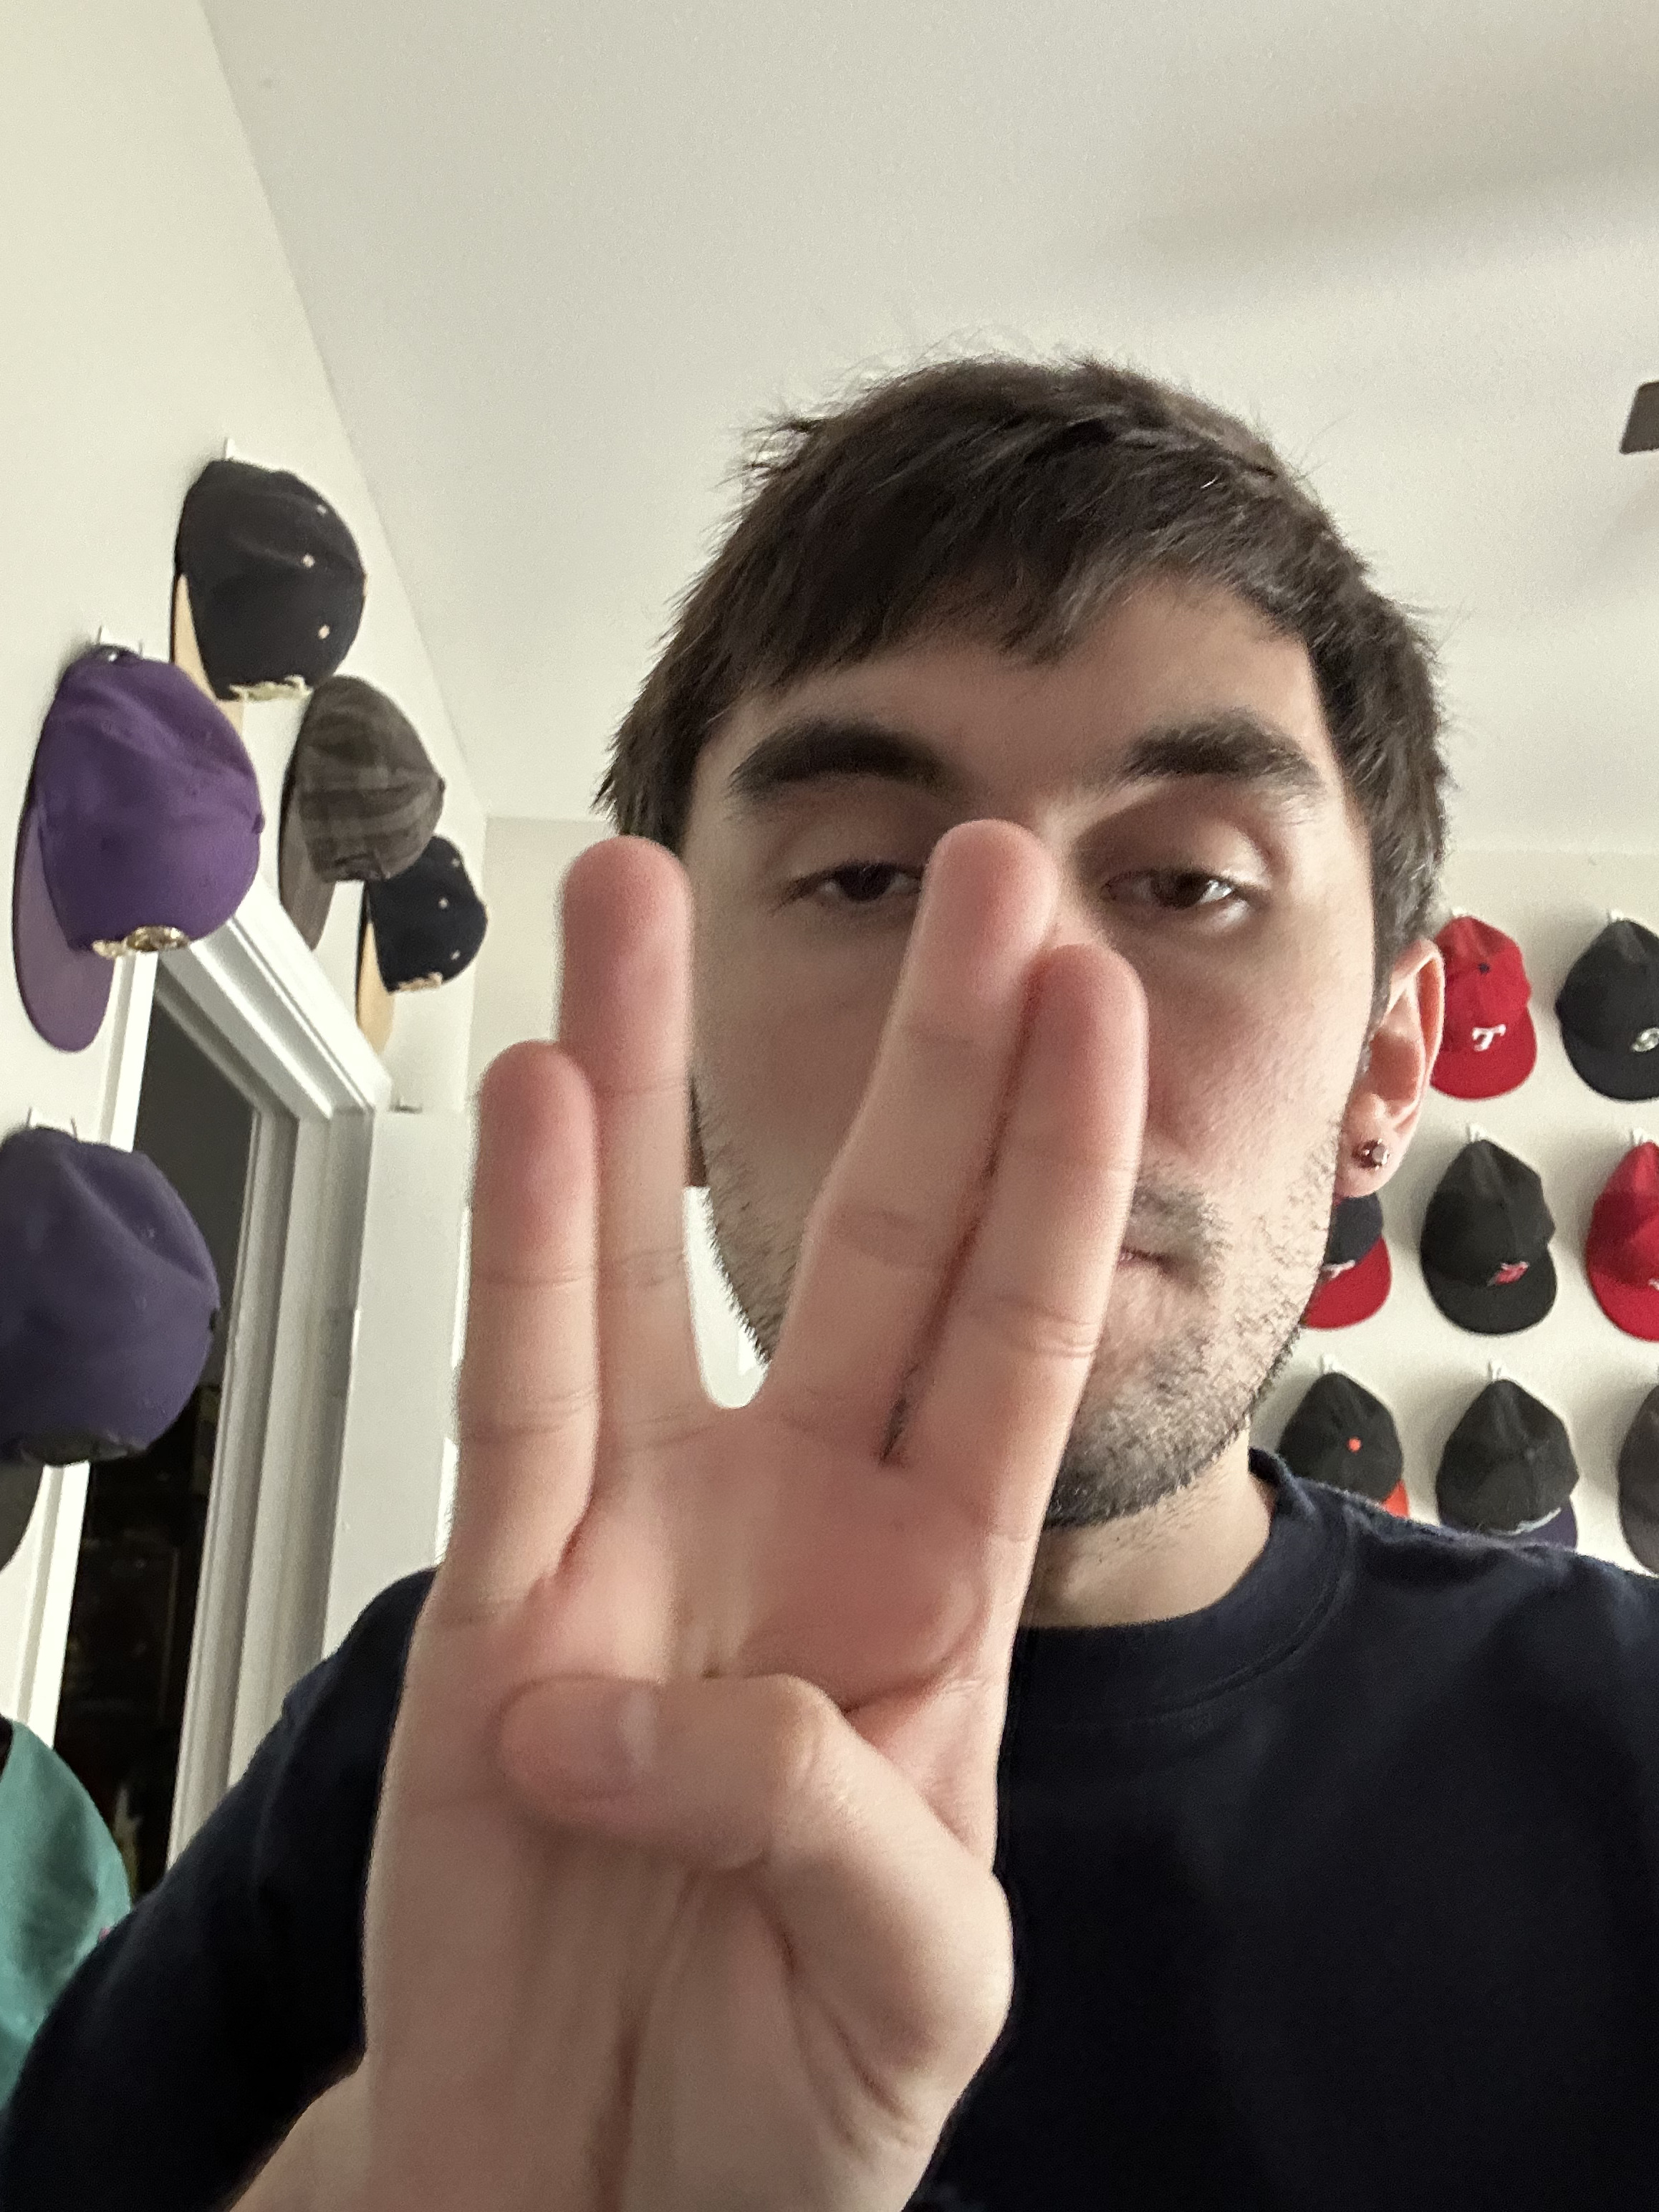
\includegraphics[width = 0.30\textwidth]{./Images/Model 2/Training Images/Spock.jpg}
            \end{center}

            During the training aspect, I rotated my hand around and moved the hand around the camera so that it was in different locations. I wanted to rotate my hand around in different orientations
            so that the model would be trained in a way that it could potentially identify differences that were drastic from the typical orientation.

            After training the model I tested it with just static hand signs that were used in the model. The model was able to identify the peace sign and Spock hand gesture relatively easily and with
            high confidence. For instance, when I held up the peace sign the model was able to identify it as the peace sign with around 99 \% confidence and the spock sign was identified with around a
            90 \% confidence rate. Interestingly enough, the model had a lot of difficulty identifying the rock and roll hand gesture. I had to try very hard to get a confidence rate that indicated that
            the model was accurately identifying the hand gesture.

            After testing the model with static images I decided to change between static images (as in I wasn't moving my hand) and moving my hand around the screen. This test had similar results to when
            I just held my hand in a static position in front of my webcam. The main difference between the static test and the movement test was that it for some reason was more accurate in identifying
            the rock and roll hand gesture. Before the model was really struggling with identifying just static hand gestures (primarily the rock and roll hand gesture). This might be because I trained the
            model by continuously changing where my hand was relative to the camera.

            The last test that I did was that I changed between specific hand gestures to others. This test yielded a myriad of different results. Mainly, the model had a really hard time identifying the
            differences between the rock and roll hand gesture and the peace sign. The model was really good at identifying the peace sign regardless of what the original hand gesture was. The other hand
            gestures were more difficult to identify, and this is probably because some of the gestures looked so similar between one another.

            I chose to make this model because the data that I trained it with was very similar to one another. For instance, the model had a hard time identifying the difference between the peace sign
            and Spock gesture. This is largely due to the fact that in the models eyes, they look very similar. If you think about it in a critical sense the peace sign and Spock gesture look similar in 
            that they both have two vertical shapes. To the human eye, these gestures are different because one involves two fingers and the other involves four fingers. To the model these gestures look
            pretty similar because of the overarching structure of the gestures.

            After getting done with training this model I discovered that the model was not really good at identifying the differences at a large scale. This is because the training of the model was really
            non trivial because of the differences between the gestures is not really drastic in the eyes of a ML model. The faults of this model could probably be remedied by using more images in the training
            aspect of the model. 

            I am very happy that I chose to make this model because it tested the limits of the model and what it could discern. This has given me a really good sneak peak as to how ML models are created
            and how they can be improved and used in everyday life.
        \end{spacing}
        \vspace*{-0.5em}
    \end{Highlight}
\end{problem}

% Problem 3
\begin{problem}{Problem 3}
    \begin{statement}{Problem Statement}
        Put the link to your model here on page 4. Add the link to a shareable Google folder containing your training images/files. Post a link to your model on Piazza and ask your classmates to try 
        it out. Include a screenshot of your post and responses here on this page.
    \end{statement}

    \begin{Highlight}[Solution]
        The link to my model can be found here \href{https://teachablemachine.withgoogle.com/models/dkkzS5pWK/}{Hand Gestures Model}. \vspace*{1em}

        Here is my post and the response(s) that I got.

        \begin{center}
            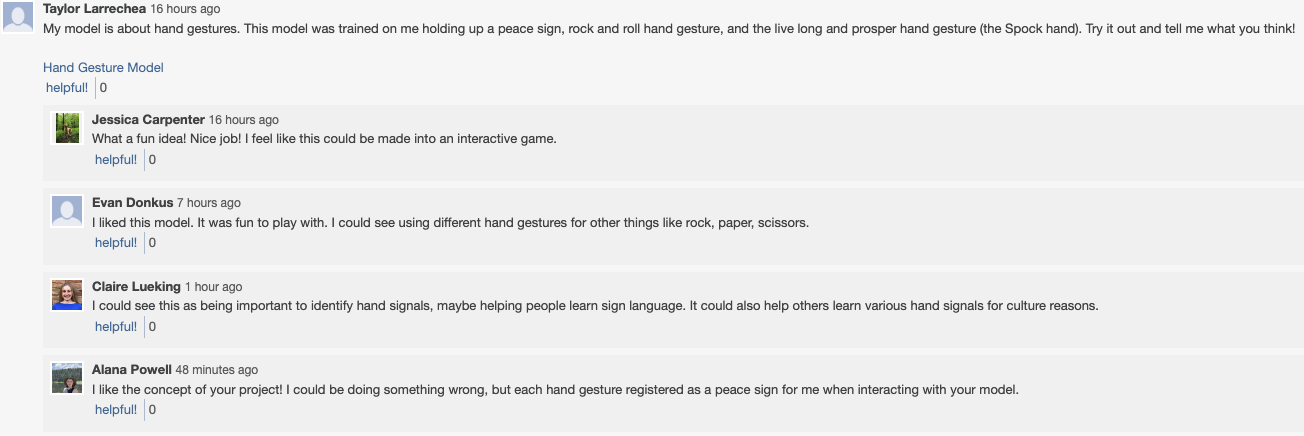
\includegraphics[width = 1.0\textwidth]{./Images/Piazza/Responses.png}
        \end{center}
    \end{Highlight}
\end{problem}

% Problem 4
\begin{problem}{Problem 4}
    \begin{statement}{Problem Statement}
        Go to Piazza and try out 3 of the models from your classmates. On the following pages, give a one page review of each (on pages 6/7/8) (may include thumbnails):
        \begin{itemize}
            \item Is the model non-trivial?
            \item What did you use to test it?
            \item How well does it work?
            \item Why is it a meaningful model?
            \item Does it do something that is hard for a human to do?
            \item What images did you use to test the other's models?
        \end{itemize}
    \end{statement}

    \clearpage
    \begin{statement}{4A Model Review One:}
        Provide the review of the 4A model.
    \end{statement}

    \begin{Highlight}[Solution]
        \begin{spacing}{1.50}
            The first model that I reviewed was by Claire Lueking. Her model was a model that tested the suits of cards. 

            \begin{itemize}
                \item \textbf{Is the model non-trivial?} - I would not classify this model as trivial. Because of the ambiguity of the suits of cards, it would be very hard to have a model that is 
                trained where it can correctly identify the suit of a card.
                \item \textbf{What did you use to test it?} - I used a deck of cards to test this model. I went through my deck of cards and held up different card values (2s, 3s, Aces etc.) with
                different suits of the cards. For example, I held up an Ace of Clubs and an Ace of Spades and the model correctly identified the suits of the cards. The same was done for other card
                values.
                \item \textbf{How well does it work?} - Overall, the model did a really good job at identifying the different suits of cards. The only critique that I have of the model is that Claire
                might have inaccurately labeled the model. For instance, as someone who has played a lot of card games (and I developed a Blackjack game) I know with all of my heart what a Club, Diamond,
                Hearts, and Spade are. When I held up a card that had a Spade as the suit, it was labeled as a Club and when I held up a Club it identified it as a Spade. I think this is not the fault of
                the model itself, it must of been because Claire incorrectly labeled the suits. Other than that it worked really well and was very accurate.
                \item \textbf{Why is it a meaningful model?} - I think this is a meaningful model because it could be used in other contexts. For example, one could make a card counting ML model that
                helps players count cards to gain an advantage. It also could be used in the context of casino security for checking what cards were on the table when controversy arrives at the table.
                \item \textbf{Does it do something that is hard for a human to do?} - Although I find this model to be useful, it doesn't do something that a human cannot do. This model may be accurate
                but an experienced card player can identify the suits of cards with rather ease.
                \item \textbf{What images did you use to test the other's models?} - I didn't use any images, I held up cards to my webcam to test the model.
            \end{itemize}
        \end{spacing}
        \vspace*{-0.5em}
    \end{Highlight}

    \clearpage
    \begin{statement}{4A Model Review Two:}
        Provide the review of the 4A model.
    \end{statement}

    \begin{Highlight}[Solution]
        \begin{spacing}{1.50}
            The second model that I reviewed was by Evan Donkus. His model was a model that tested if a plant was poison ivy or not.

            \begin{itemize}
                \item \textbf{Is the model non-trivial?} - I think the model is non trivial. To the naked eye of a lot of people most would probably have a hard time discerning what is and isn't poison
                ivy. I think most people can identify that a plant is safe to touch, like a four leaf clover, but they may struggle with actually identifying poison ivy.
                \item \textbf{What did you use to test it?} - Because I don't really know what poison ivy looks like, I went to Google and looked for images of poison ivy. I then went and grabbed an image
                of a four leaf clover. I then fed the images to the model and tested if the model could accurately identify the image that I fed to it.
                \item \textbf{How well does it work?} - From what I saw, the model is actually not that accurate. Going straight to Google and finding an image of poison ivy it did not say that it was 
                poison ivy. On the contrary, when I fed the model a picture of a four leaf clover it identified it as poison ivy. Having seen the results from the first test I can see that it might actually
                need more training data to be accurate.
                \item \textbf{Why is it a meaningful model?} - Even with its inadequacies, I think this model would be really useful especially for outdoors type people. Say you are on a hike, and you want to
                know if something is dangerous to come in contact with. This model would be the perfect for that type of use. I believe with more training data it could be a very useful model in a lot of
                contexts.
                \item \textbf{Does it do something that is hard for a human to do?} - Unlike some other models I think this is something that most humans cannot do. I don't think the average person is good
                at determining if something is poison ivy or not. So because of this, I would say that this model does something that most humans cannot do.
                \item \textbf{What images did you use to test the other's models?} - As mentioned previously, I went to Google and found an image of poison ivy and a four leaf clover. I then fed this into the
                model and viewed the results.
            \end{itemize}
        \end{spacing}
        \vspace*{-0.5em}
    \end{Highlight}
    
    \clearpage
    \begin{statement}{4A Model Review Three:}
        Provide the review of the 4A model.
    \end{statement}
    
    \begin{Highlight}[Solution]
        \begin{spacing}{1.50}
            The third model that I reviewed was by Jessica Carpenter. Her model was a model that tested if a banana was unripe, ripe, or rotten.

            \begin{itemize}
                \item \textbf{Is the model non-trivial?} - I think this model errs more on the trivial side. But depending on the person it may be non trivial. I am someone who doesn't really know 
                when a banana is necessarily rotten, but I do know when a banana is unripe. Trying to figure out when a banana is ripe is kind of hard but to a trained eye it can be kind of easy.
                \item \textbf{What did you use to test it?} - I went to Google and found images of unripe, ripe, and rotten bananas. I then fed this to the model and looked at how well it identified
                the stages of the bananas.
                \item \textbf{How well does it work?} - The model works pretty well, however it doesn't work as well as a humans eye does. For instance, when I fed it an image of a clearly rotten banana
                it gave only a 80 \% confidence rate that it was rotten. The other 20 \% was in the unripe classification. I also tested it with a ripe banana and it came back that the banana was rotten.
                \item \textbf{Why is it a meaningful model?} - This could be a meaningful model in helping people determine when to throw out bananas because they are rotten. It also could be really helpful
                in determining when you could use them to make something like yummy banana bread!
                \item \textbf{Does it do something that is hard for a human to do?} - Depending on the person, this model doesn't really do something that a human can't do. For instance, if someone is
                really good with baking, they may be good at identifying if a banana is ripe or not. The average person may or may not be able to do this but it really depends on the person.
                \item \textbf{What images did you use to test the other's models?} - As mentioned previously, I went to Google and found images for the stages of bananas. I then fed this to the model
                and looked at the results.
            \end{itemize}
        \end{spacing}
        \vspace*{-0.5em}
    \end{Highlight}
\end{problem}